\chapter{Introduction\label{intro}}

\textcolor{red}{use the word public license instead of PCL, make fixes per perens' other comments. Free software license != strong copyleft software license
}

PCLs play a central role to the distribution of works in software engineering. For example in open source there must be an appropriate PCL attached to the source code in order for the piece of software to be freely available for possible modification and redistribution. Because open source is central to software engineering the licenses enabling open source must also be considered important in the same context.

Public license is defined by Wikipedia with the following words \citep{wikipedia:publiclicenses}:
\begin{quote}
	''A public license is a copyright license where the licensees are not limited. Examples include free content, open content, Creative Commons, free software and open source licences.''
\end{quote}

Understanding PCLs can be difficult. This could stem from the legal nature of the license texts and the large number of already-existing PCLs. The license texts usually favors correctedness over the readability for the developer. This is because the license text has to act as a valid legal instrument otherwise it cannot be endorsed \citep{ferguson2006gpl}. The lack of understanding of PCLs leaves too much room for interpretation. In June 21, 2023 International Business Machines' (IBM) Red Hat seemingly violated a PCL, the GNU General Public License version 2 (GPL-2.0) \citep{sfc:rhel} \citep{ibm:rhel}. This was an unpleasant surprise to the public since the project behind GNU General Public License (GPL), GNU Project initially attempted to ensure the users via the GPL have to the following three freedoms \citep{gnu:free}:
\begin{itemize}
	\item Freedom 1:	The freedom to study how the program works, and change it so it does your computing as you wish. Access to the source code is a precondition for this.
	\item Freedom2: The freedom to redistribute copies so you can help others
	\item Freedom 3:	The freedom to distribute copies of your modified versions to others. By doing this you can give the whole community a chance to benefit from your changes. Access to the source code is a precondition for this.
\end{itemize}

Regardless, IBM's Red Hat essentially rendered the previously public Red Hat Enterprise Linux (RHEL) into proprietary software. If the licenses would be more easily understood the proprietarization of RHEL would have been less of a surprise to the users.

On top of PCL details, software engineers in general have a tough time understanding the basic goals of PCLs used in software engineering. In the instance of the RHEL incident it would not have been a big surprise to software engineers if they would have known about other licenses and what they try to achieve or how old is GPLv2 and why it has been succeeded by GNU General Public License version 3 (GPL-3.0).

This thesis' goal is to contribute into the solving these problems in a structured manner. First we state definitions and terminology used in the scope of this thesis. We go over the reasons why there does not exist consistent terminology in this area and why the conversely the definitions are the most stabile ones in this area. Second we take a deep dive into the PCLs through a multivocal literature review. To make more information available, a mapping study connected to the terminology scope defined in the first step is needed. Third includes our own suggestions and basic knowledge for professionals and academics in the industry to enhance the understanding of PCLs in software engineering. This step also includes discussion of the future research and contributes to stablizing the terminology and reinforcing the already-existing definitions in the academic field.

\section{Research goal, questions and contributions}
The primary goal of this research is to conduct a multivocal literature review of the current state of PCLs in software engineering, the evaluation of the them and the evidence level of the research. The research aims to provide a novel perspective on relevant licenses and to extract key findings through a rigorous literature review process. The research questions of the review are:
\begin{itemize}
	\item RQ1: How many PCLs in software engineering does there exist?
	\item RQ3: What is the average length of a PCL in software engineering?
	\item RQ3: What are the most common components seen in PCLs in software engineering?
	\item RQ4: What are the most common changes made to PCLS in software engineering?
\end{itemize}

Terms such as open source, source code, software freedom and other vocabulary must be defined in the scope of this thesis. \hyperref[sec:bg]{Section 1.3} will examine this plethora of of terminology and definitions and will be used to establish a sound basis for discussing this broad subject.

This study has two main viewpoints. The first one is to provide rigorous multivocal research on PCLs to the academic field. Because this thesis already does the multivocal work on PCLs in software engineering the researches of the future can cite the results of this thesis without having to mark their study a multivocal one. This is the grand goal of this thesis. The second one is to provide insights and general metrics to the professional field of software engineering on PCLs. Hopefully this makes conversation on PCLs in software engineering easier and more rooted to scientific research rather than gut feeling and old, non-scientific articles on the insights and metrics of PCLs in software engineering.

\section{Thesis structure}
This thesis follows the IMRaD structure. \hyperref[intro]{Chapter 1} introduces the problem, this thesis' possible contributions and some further background. \hyperref[methods]{Chapter 2} goes over the process and the methods of the multivocal literature review. This is where most of the actual research takes place in. \hyperref[results]{Chapter 3} presents results to the research questions. \hyperref[discussion]{Chapter 4} discusses implications for research. The chapter also discusses software engineering professionals in the thesis' context and the validity of the thesis' research. \hyperref[conclusions]{Chapter 5} concludes this thesis with the help of the research questions and the future of the research.

\section{Background and terminology of PCLs}
\label{sec:bg}
The current terminology is used with different definitions which leads to inconsistencies in the field of software engineering. For example The Open Source Initiative (OSI) classifies GPL-3.0 under the term ''open source'' whereas the Free Software Foundation (FSF) classifies GPL-3.0 under the term ''free software'' \citep{osi:gplv3}\citep{rms:opensource}. This is because their definitions on open source and free software differ from each other. Some parts of the two definitions are even mutually exclusive. This is rarely mentioned when people talk about Free and Open Source Software (FOSS) or Free / Libre and Open Source Software (FLOSS) which leads to misunderstanding that the two approaches are the same. This is why our focus will be PCLs in software engineering, which distinguishes our investigation from the broader topic of PCLs or the copyright law. This includs also PCLs that are not approved by the FSF nor OSI hence not falling under the group of FLOSS licenses. The term ''copyleft'' is defined by \cite{mustonen2003} in the following way:
\begin{quote}
	''Copyeft is a novel licensing scheme. It facilitates open and decentralized software development. Its key feature is that once a program is licensed by the inventor, the subsequent programs based on the original must also be licensed similarly.''
\end{quote}
This is why the term is often used in the context of free software.

In this section we aim to increase the accessibility of our discussion by providing  a concise overview of the background of the field of PCLs and the terms we employ.

To explain our emphasis on PCLs in software engineering, it is essential to examine the other possible areas of interest in PCLs. Our study classifies such efforts into eight domains as mentioned by the GNU Project \citep{gnu:licenselist}.

These domains include:
\begin{itemize}
	\item PCLs in software engineering
	\item PCLs in documentation for example architecture documentation of a project that may or may not be software or even publicly licensed
	\item PCLs in artistic works for example digital art, music or videos
	\item PCLs in educational works
	\item PCLs in fonts
	\item PCLs in viewpoints
	\item PCLs in physical objects
	\item PCLs in other works
\end{itemize}

The primary aim of this study is to investigate PCLs in software engineering process. However, it is important to acknowledge that PCLs in software engineering are only aspect of PCLs. These additional dimensions are crucial in adoption and implementation of PCLs in software engineering, but they are not the focus of this thesis.

For example, including artistic works such as music would require us to understand the basics of music theory and what sets apart distinct pieces of music from one another, something that could be outside the skillset of the author. While developing a comprehensive theory, framework, and tooling for PCLs as a whole is a gargantuan task beyond the scope of a single thesis, narrowing our focus to software engineering enables us to examine a more concise and complete aspect of the main topic of this thesis. 

As significant point of clarification, it is essential to acknowledge that PCLs are generally meant to be used as valid legal instruments. The question whether or not a PCL can act as a legal instrument is critical to the main function of these licenses. However, this thesis will not focus on the legal doctrine aspects either. The enforceability of PCLs has seen discussion in the academic field of law since the dawn of PCLs and since there's already an academic base for research it is likely the discussion seems to continue on with a healthy amount of activity \citep{duisburg2011gpl}.

Since the most recognized PCLs in software engineering in public are either open-source licenses or free-software licenses and since both paradigms are driven by different organizations with very different goals and values, it is understandable how non-standardized the terminology in the scope of PCL in SE is. The example given in the first section of this sub-chapter illustrates the challenges involved in maintaining consistency in the use of terminology in this emerging field and further warrants a closer inspection of the terminology to emphasize our own standing in the field.

To provide an understanding of the terminology used in this thesis, a Venn diagram is presented in \hyperref[fig:terms]{Figure 1.1}, which contextualizes the non-standardized terminology within the PCL scope as a whole. This perspective provides an increased understanding of where different subdomains fall in the larger picture of PCLs. Furthermore it is essential to note that PCLs in software engineering encompasses different aspects that require a closer examination.

\begin{figure}[t]
	\centering
	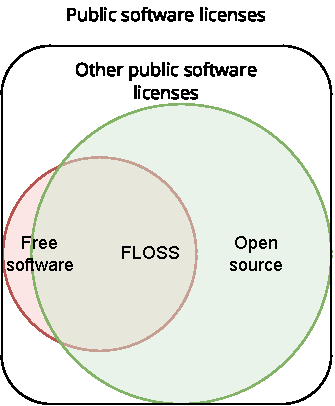
\includegraphics[scale=1.5]{figures/terms-diagram.pdf}
	\caption{PCLs in software engineering}
	\label{fig:terms}
\end{figure}

Let us explore further the differences and similarities between open source and free software at the software engineering level of PCLs. This is a crucial step since we can see from the approximation in \hyperref[fig:terms]{Figure 1.1} that the majority of PLCs are either free software, open source or both. We glanced over the free software definition in the first section of \hyperref[intro]{Chapter 1}. Open Source Initiative defines open-source licenses in the Open Source Definition briefly in the following way \citep{osi:licenselist}:
\begin{quote}
	''Open source licenses are licenses that comply with the Open Source Definition - in brief, they allow software to be freely used, modified, and shared.''
\end{quote}

Like the FSF with free software, OSI has the final word on what passes as open source and what does not. For example a new software PCL will not classify as free software nor open source until the corresponding organization has acknowledged the software PCL as either free software, open source or neither. If a PCL is accepted by both FSF and OSI it will fall under the term FLOSS. If a PCL gets accepted by neither of the organization or it gets rejected by both organizations it will fall under other software PCLs in the \hyperref[fig:terms]{Figure 1.1}. In general free software license requirements are considered more strict than the open source license requirements. For the sake of perspective we could simplify the differences like so: free software requires the redistributions of the licensed software to be open as well but open source does not require this. The terms free software and open source are in general often misunderstood or just thought of as FLOSS collectively because the terms have a hard time conveying their paradigms in the natural language. One would not think free software does not mean software free of charge nor would one think that open source allows closed source redistributions of the licensed software. We will glance over the impacts on the industry of these two terms in \hyperref[discussion]{Chapter 4}.

With the context laid out in this chapter let us define PCLs in software engineering for the purpose of this study: Public software licenses are copyright licenses where the licensees are not limited and the copyright license in question is meant be used in licensing software source code. This helps us create the search strings and find the relevant literature for this thesis. This also helps us exclude PCLs regarding documentation, media and all other non-software targeted PCLs.

The quest to categorize every software PCL under some paradigm objectively is a complex one and cannot be comprehensively answered in a single paragraph. Therefore it is essential to continue taking the correct steps towards incresing the scientific understanding and providing the industry with examples, standards and processes to follow. However, as the following chapters reveal, a significant amount of effort is still being spent on solving the same problem multiple times, rather than building on existing knowledge and finding the next problem to solve. This thesis aims to contribute to mitigating this challenge by providing a rigorous analysis of the current state of the field. As the knowledge, conventions, and terminology take shape,we can look forward to reaching a state where less effort is spent on defining concepts and more on practical problem-solving.